\documentclass{article}

\usepackage{graphicx}
\usepackage{subfigure}
\usepackage{epstopdf}
\usepackage{float}
\usepackage{url}

\hyphenation{op-tical net-works semi-conduc-tor}

\begin{document}

\title{Thesis Report}
\maketitle

\section{Introduction and Background}

We would use existing solver as a black-box to build upon and call it as subroutine. Our new solver's search strategy would be guided by the structure and call IDP to solve subproblems.

\section{Design Frame}
Eclat is a program to find frequent item sets (also closed and maximal as well as generators) with the Eclat algorithm~\cite{zaki1997new}, which carries out a depth first search on the subset lattice and determines the support of item sets by intersecting transaction lists.

The design frame is showed in Figure~\ref{fig:frame}. Given the data which could be a set of graphs, sequences, and transactions, after a user giving inputs which include the type of problem to solve, the matching pattern, the constraints of the problem, and the dominance. 

\begin{figure}
\centering
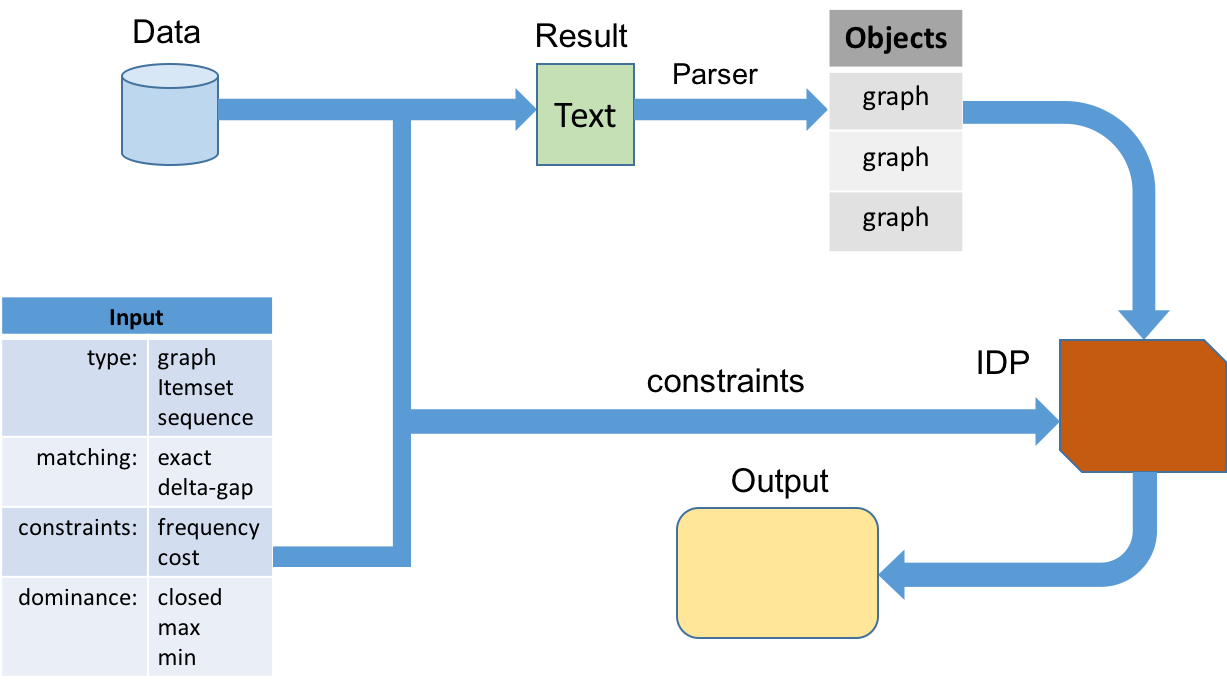
\includegraphics[width=0.75\textwidth]{figures/structure.png}
\caption{Design frame.}
\label{fig:frame}
\end{figure}

\begin{itemize}
\item Use gSpan~\cite{yan2002gspan} or eclat~\cite{zaki1997new} to get frequent patterns (frequent graphs or itemsets).

\item Use Parser method to get python objects from frequent patterns in text.

\item Given these frequent graphs or itemsets and user inputs (especially constraints), use IDP~\cite{de2014predicate} to find results (such as, closed itemsets) from python objects.
\end{itemize}

\bibliographystyle{IEEEtran}
\bibliography{report}

\end{document}